\chapter{Results and discussion}
\label{ch:results}

This chapter reports what was built and measured, and discusses why the results
should be believed. It covers correctness testing, then computation cost, then
communication cost with the component breakdown, and finally the application
demonstration.

\section{Correctness and robustness}
\label{sec:res-correctness}

Before any performance claim, the implementation must be shown to be \emph{correct}.
An adaptor signature is not correct merely because it signs and verifies; it must
satisfy a specific contract, and a consolidated harness (\texttt{test\_contract})
checks every clause of that contract and prints each as a labelled pass. \Cref{tab:contract}
lists the checks and their outcomes.

\begin{table}[t]
  \centering
  \caption{The adaptor-signature correctness contract, each clause checked and passed
  by \texttt{test\_contract} (corroborated at scale by the 1000-iteration functional
  suite on modes 2/3/5, the 256-instance serialization suite, and the pinned
  known-answer test).}
  \label{tab:contract}
  \begin{tabular}{@{}llc@{}}
    \toprule
    \# & Property & Result \\
    \midrule
    1 & PreSign produces a pre-signature that PreVerify accepts & pass \\
    2 & the pre-signature \emph{fails} basic Verify (statement-binding tripwire) & pass \\
    3 & Adapt yields a signature that basic Verify accepts & pass \\
    4 & Extract recovers the witness \emph{exactly} ($y'=y$) & pass \\
    5a & a tampered message fails Verify & pass \\
    5b & every single bit-flip of the packed signature is rejected & pass \\
    6 & malformed packed bytes are rejected ($pk\!\ge\!Q$, ternary code-3, $z$ out of band) & pass \\
    7 & the deterministic API is byte-identical on re-run & pass \\
    \bottomrule
  \end{tabular}
\end{table}

Each clause matters. Clauses~1--4 are the adaptor contract itself: a pre-signature is
verifiable yet unspendable (the tripwire, clause~2), becomes a basic signature
once the witness is added (clause~3), and the act of completing it reveals the witness
(clause~4) --- the mechanism that makes an atomic swap atomic. Clauses~5--6 are
robustness: the byte-level verifier an on-chain integration would consume must not
trust its input, so it rejects tampering and malformed encodings. Clause~7 is
reproducibility, which lets an independent verifier be cross-checked against fixed
vectors. All clauses pass, with zero compiler warnings under the project's strict
flags.

\section{Computation cost}
\label{sec:res-compute}

The primary, fair comparison is LAS against its own simplified base, since they share
algorithm, parameters, and primitives (\cref{sec:benchmethod}); it measures the
overhead of the adaptor layer. \Cref{tab:overhead} reports it at the project's target
setting, \emph{Simplified Dilithium-III} ($n{=}6$, $\ell{=}5$, $\kappa{=}49$;
\cref{tab:params,tab:notation}), pairing each adaptor operation with the basic
operation it mirrors; \cref{tab:overhead-levels} then confirms the same overhead at all
four settings. Each entry is the mean $\pm$ sample standard deviation over ten runs of
one thousand iterations (\texttt{bench\_levels}).

\begin{table}[t]
  \centering
  \caption{Key overhead summary at the \emph{Simplified Dilithium-III} (target) setting
  ($n{=}6$, $\ell{=}5$, $M{=}11$, $\kappa{=}49$, $\gamma{=}137\,984$, $N{=}256$,
  $q{=}8\,380\,417$); $\mu$s/op, mean $\pm$ sample SD over 10 runs $\times$ 1000
  iterations (\texttt{bench\_levels}). Overhead is each adaptor operation over its basic
  analogue; KeyGen (and statement generation) is shared by the basic signature and LAS.}
  \label{tab:overhead}
  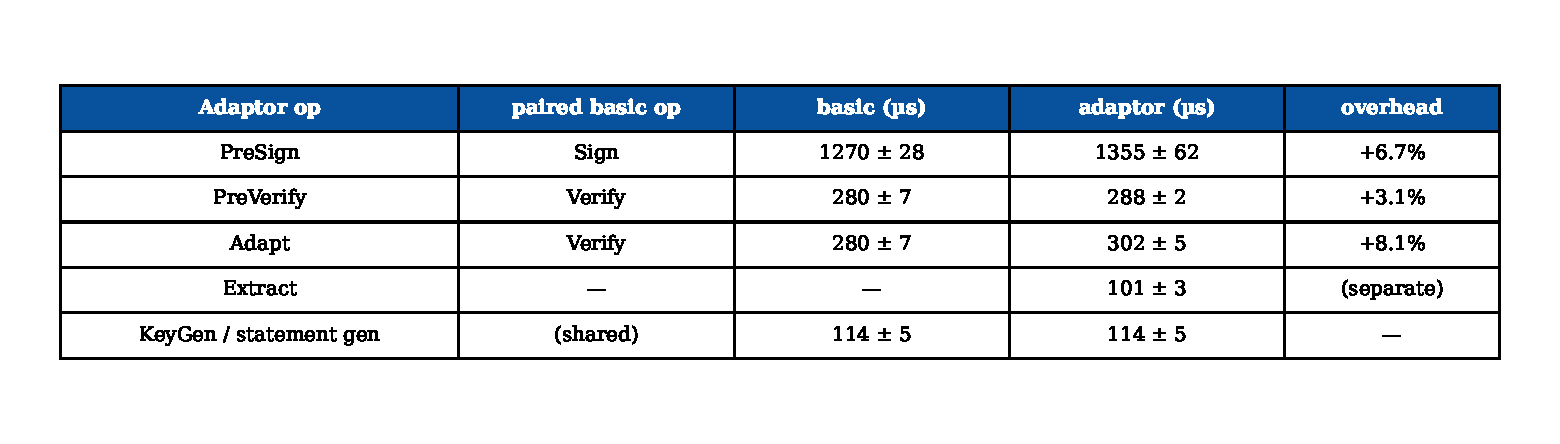
\includegraphics[width=0.9\linewidth]{figures/tab_overhead_l3}
\end{table}

The result is that the adaptor layer is almost free in computation, and the numbers
are not just small --- they are small \emph{for structural reasons}:
\begin{itemize}
  \item \textbf{PreSign $\approx$ Sign} ($+6.7\%$): PreSign runs the same masked-commit,
        hash, respond, reject loop as Sign; it only adds the statement $Y$ into the
        Fiat--Shamir commitment and rejects at a slightly tighter bound. Neither
        changes the asymptotic work.
  \item \textbf{PreVerify $\approx$ Verify} ($+3.1\%$): PreVerify recomputes the same
        commitment shape as Verify, differing only by the $+Y$ addition before hashing.
  \item \textbf{Adapt $\approx$ Verify} ($+8.1\%$): Adapt first runs a PreVerify and
        then adds the witness vector, so it costs about one verification plus a few
        polynomial additions.
  \item \textbf{Extract is cheapest and reported separately}: it has no basic analogue;
        it only subtracts $z-\hat z$ and checks $A\,y=Y$.
\end{itemize}

This overhead is stable across security levels. \Cref{tab:overhead-levels} repeats the
measurement at each parameter set: the adaptor premium stays in the single digits ---
at most about eight percent --- everywhere, so adding adaptor functionality does not
become more expensive as the scheme is scaled up.

\begin{table}[t]
  \centering
  \caption{Adaptor overhead is small at every parameter set (\texttt{bench\_levels};
  mean over 10 runs $\times$ 1000 iters, Extract in $\mu$s). Percentages are each
  adaptor operation over its basic analogue.}
  \label{tab:overhead-levels}
  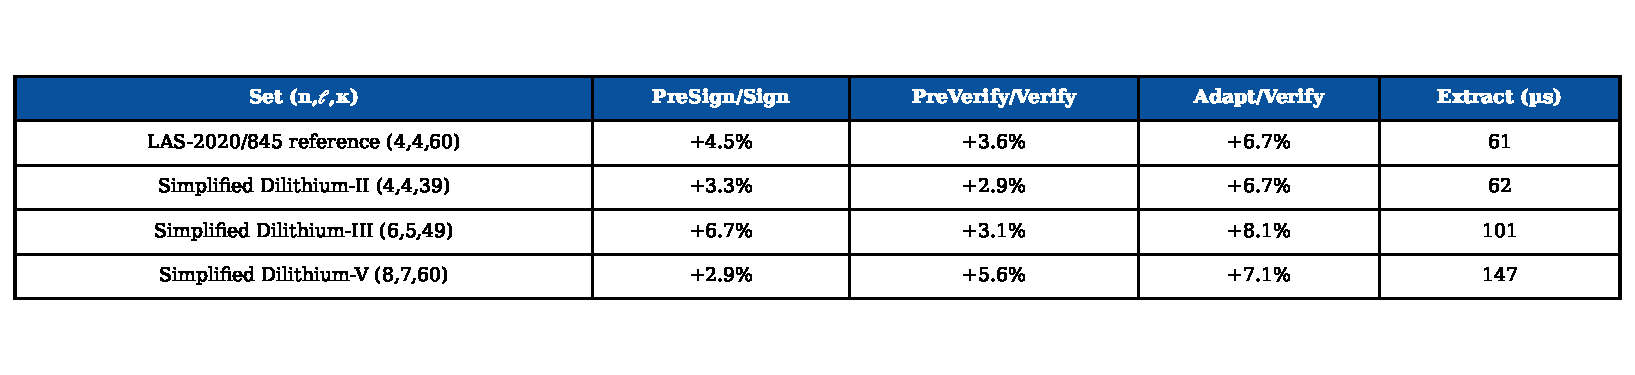
\includegraphics[width=\linewidth]{figures/tab_overhead_levels}
\end{table}

Signing and pre-signing are dearer than verification because they use rejection
sampling. The acceptance rate was measured directly, by counting rejection-loop
attempts rather than estimating from a timing ratio: at every setting approximately
37\% of attempts are accepted, so a signature takes about 2.7 attempts on average. This matches the closed-form prediction: one attempt is accepted only if
all $(n+\ell)\cdot N$ response coefficients fall within the bound, giving a per-attempt
acceptance of $(1-\kappa/\gamma)^{(n+\ell)N}\approx e^{-1}\approx 36.8\%$. Rejection
sampling is intrinsic to the Fiat--Shamir-with-aborts family, not a defect of this
implementation.

\section{Communication cost and component breakdown}
\label{sec:res-comm}

The computation results above show the adaptor layer is cheap. The size results show
where the real cost lies. \Cref{tab:components} decomposes every LAS object into its
components, in actual packed bytes (by the field-width formula the serializer uses),
across the parameter sets. The aim is to explain \emph{which} component drives the
size, not merely to state that signatures are large.

\begin{table}[t]
  \centering\small
  \caption{LAS objects by component (packed bytes; \texttt{bench\_levels}). The
  LAS-2020/845 reference set shares the Simplified Dilithium-II dimensions. The
  challenge $c$ is fixed; the response $z$ grows with $n+\ell$ and dominates the
  signature at every setting.}
  \label{tab:components}
  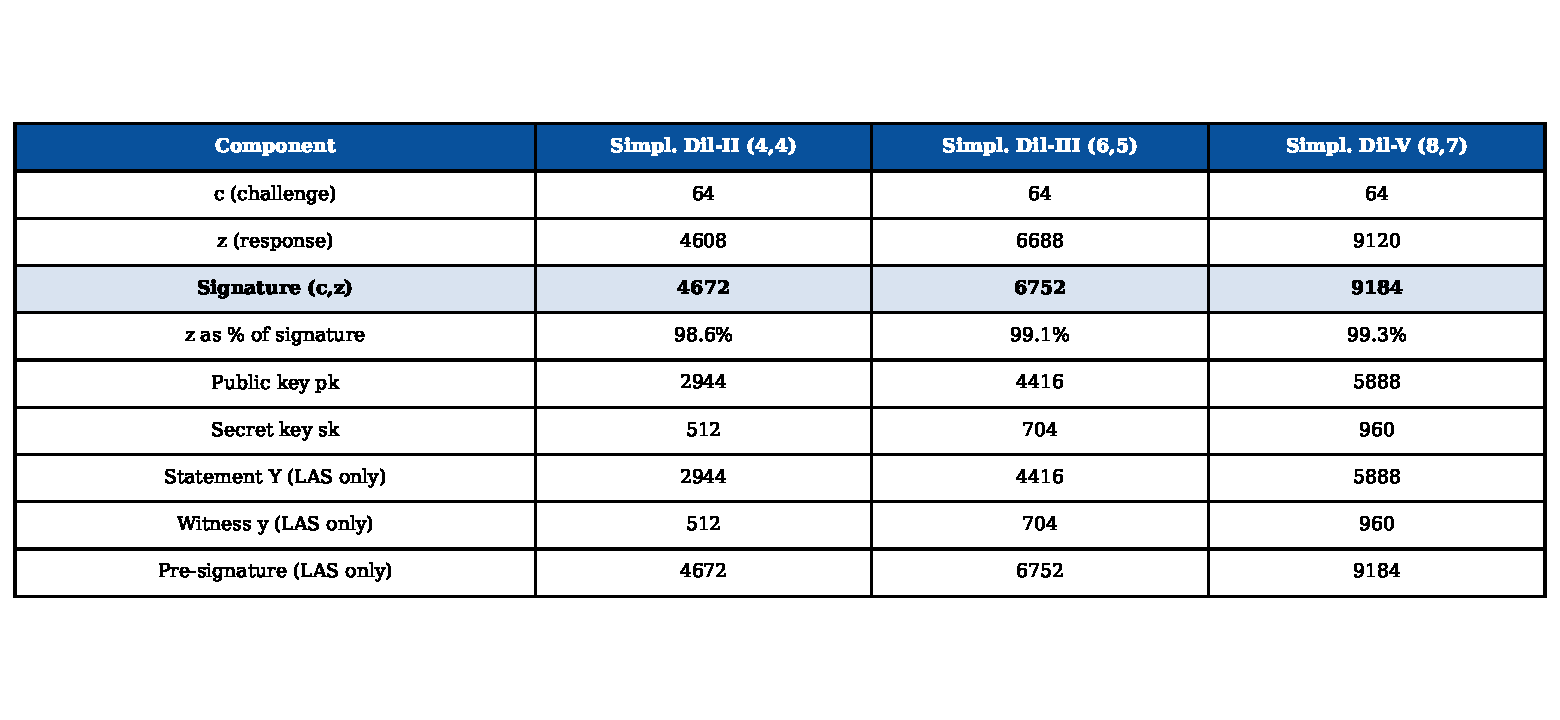
\includegraphics[width=0.85\linewidth]{figures/tab_components}
\end{table}

Two points follow, and together they give the sharp conclusion of the evaluation:
\begin{itemize}
  \item \textbf{The response $z$ is essentially the entire signature} --- 98.6\% at
        Simplified Dilithium-II, rising to 99.3\% at Simplified Dilithium-V. The
        challenge $c$ is a fixed 64 bytes and
        is irrelevant to size. Any optimisation of LAS signatures is an optimisation
        of $z$.
  \item \textbf{An adaptor swap additionally transmits a public-key-sized statement
        $Y$ and a signature-sized pre-signature}, while the witness is small. These are
        the only objects an adaptor protocol sends that a basic signature does not.
\end{itemize}

\noindent\textbf{The sharp conclusion: the cost of LAS is not adaptor computation but
communication --- specifically the response vector $z$ and the statement $Y$.} The
preceding section showed the adaptor operations add at most about eight percent of
compute over the basic scheme; this section shows the objects that move on the wire are
one to a few kilobytes, dominated by $z$. For a blockchain setting, where every byte is
stored and replicated, this is the property that matters, and it is a far more useful
statement than ``the signature is 4672 bytes''.

The response is stored at its full width: each coefficient occupies 18--19 bits
(\cref{tab:components}) rather than being range-reduced or entropy-coded. This is the
clearest opportunity for reducing the on-wire footprint, since compressing $z$ would
shrink the signature, pre-signature, and settlement payload together; it is left as
future work (\cref{sec:future}).

For a single reference point, \cref{tab:complete-l3} consolidates \emph{every}
communication object and \emph{every} protocol operation at the target setting next to
the basic signature, so the complete cost of the adaptor layer can be read in one
place: the key pair and KeyGen are shared, the four adaptor operations add single-digit
time overhead, and the only extra objects on the wire are the public statement $Y$ and
the signature-sized pre-signature.

\begin{table}[t]
  \centering\small
  \caption{Complete LAS vs.\ basic-signature comparison at the \emph{Simplified
  Dilithium-III} (target) setting ($n{=}6$, $\ell{=}5$, $M{=}11$, $\kappa{=}49$,
  $\gamma{=}137\,984$, $N{=}256$, $q{=}8\,380\,417$). \emph{Top:} communication ---
  packed bytes of every object. \emph{Bottom:} computation --- $\mu$s/op, mean $\pm$
  sample SD over 10 runs $\times$ 1000 iterations (\texttt{bench\_levels}). ``Basic'' is
  the simplified Dilithium-style base signature; shared rows are byte- or
  cycle-identical in both. The adapted signature is itself a valid basic signature.}
  \label{tab:complete-l3}
  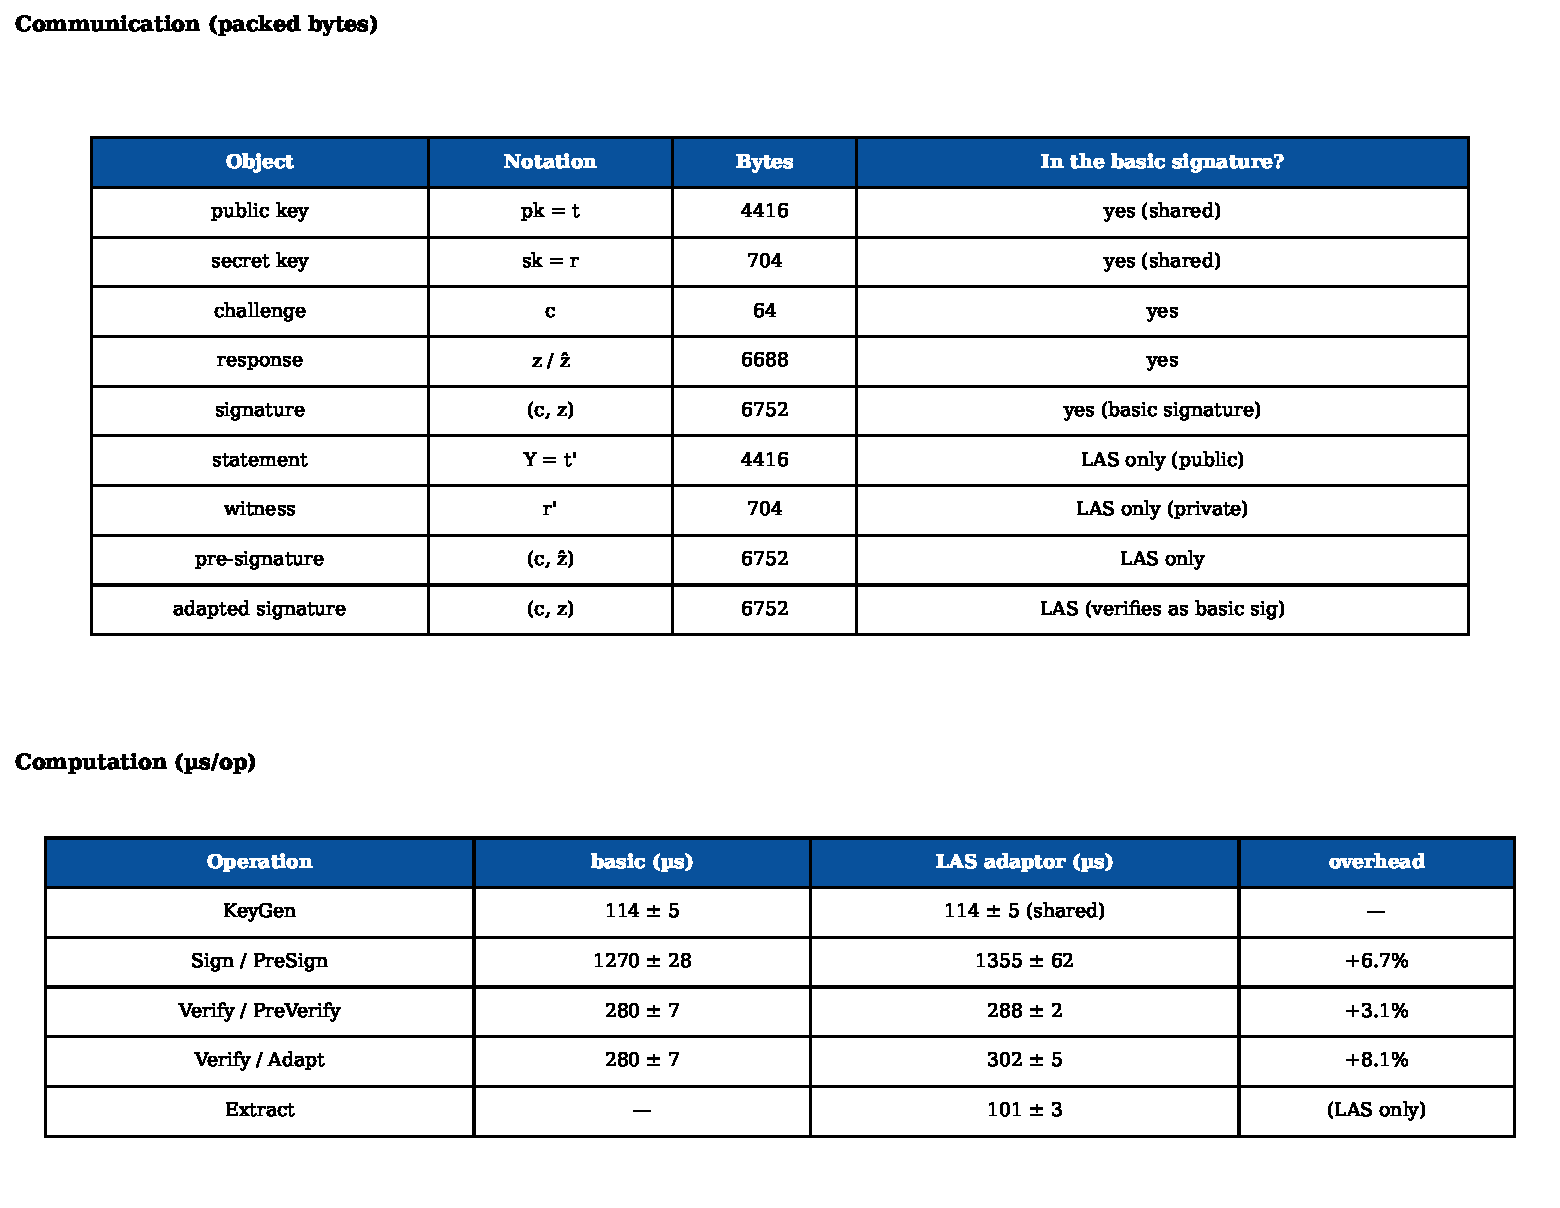
\includegraphics[width=0.95\linewidth]{figures/tab_complete_l3}
\end{table}

\subsection{The price of post-quantum: classical adaptor baseline}
\label{sec:res-classical}

The second baseline is a classical secp256k1 ECDSA adaptor signature
\cite{secp256k1zkp}. It is the natural functional counterpart of LAS: both are adaptor
signatures with the same operation set (KeyGen, Sign, Verify, PreSign, PreVerify,
Adapt, Extract) and both drive scriptless atomic swaps. They are compared on equal
footing functionally, while differing in their security foundation: secp256k1 provides
approximately 128-bit \emph{classical} security and is not quantum-resistant, whereas
LAS rests on lattice assumptions believed to resist quantum attack. The comparison
therefore measures the practical cost of moving from a classical adaptor signature to a
post-quantum one. Plain ECDSA is not used, because the counterpart of an adaptor
signature is another adaptor signature.

For this baseline LAS is instantiated at the \emph{Simplified Dilithium-II} parameters,
and only that setting is used. The reason is that secp256k1 offers roughly 128-bit
classical security, and the nearest post-quantum target is NIST level~2 (also pitched at
the 128-bit category); aligning LAS to the Dilithium-II dimensions therefore gives the
most like-for-like security target for the classical scheme. Comparing the 128-bit
classical adaptor against LAS at the Simplified Dilithium-III or -V settings would pit
it against a deliberately stronger post-quantum configuration and would understate the
classical scheme, so the higher settings are reserved for the parameter-sensitivity
study of \cref{sec:res-compute} and not used here. \Cref{tab:classical} reports both
schemes at their adaptor operations.

\begin{table}[t]
  \centering
  \caption{Classical vs.\ post-quantum adaptor signature: same functionality, different
  security foundation. Classical secp256k1 ($\approx$128-bit classical) and LAS at the
  \emph{Simplified Dilithium-II} parameters. Timings $\mu$s/op (mean over 10 runs
  $\times$ 1000 iterations, same machine); sizes in bytes. KeyGen also produces the
  statement/witness, which take the public-key/secret-key size.}
  \label{tab:classical}
  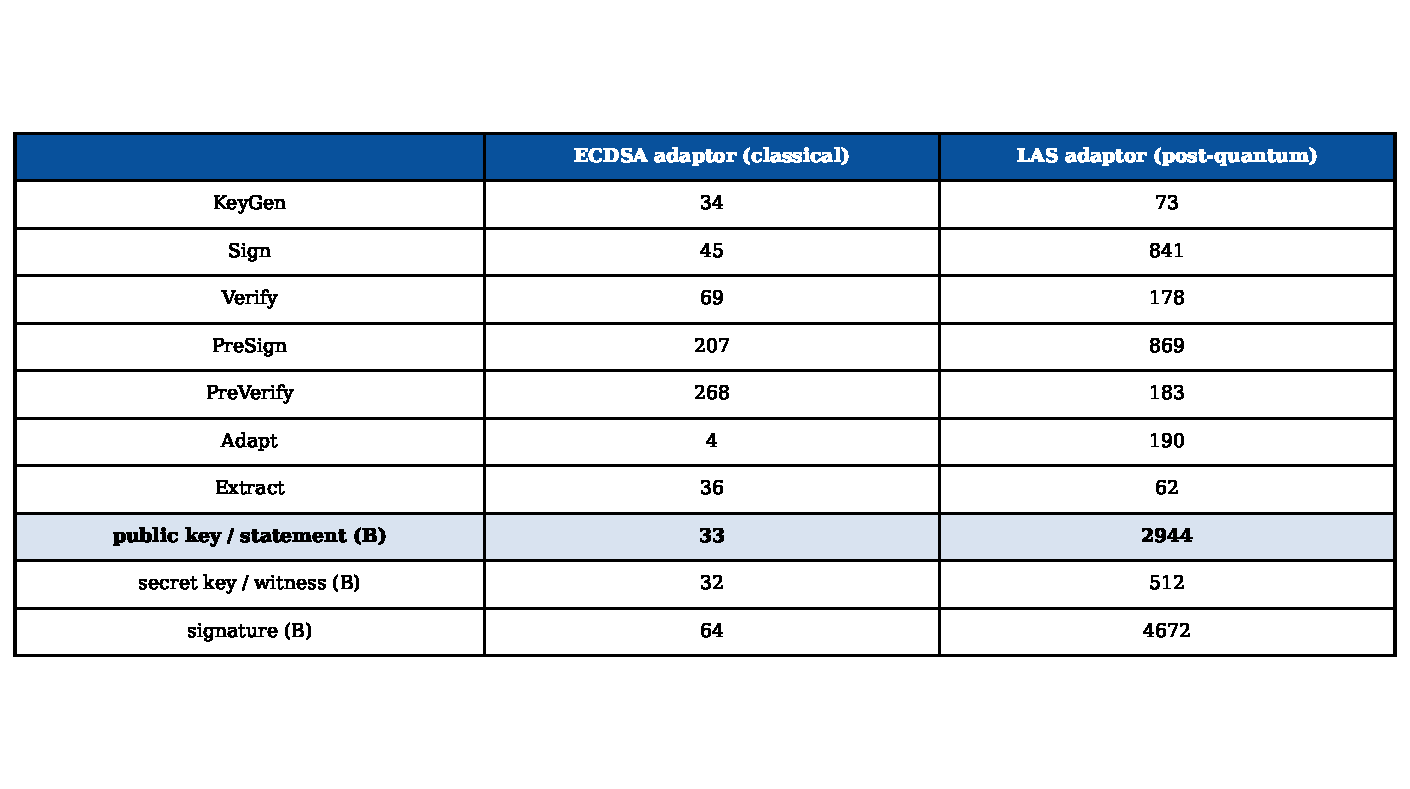
\includegraphics[width=0.72\linewidth]{figures/tab_classical}
\end{table}

This baseline compares two adaptor-signature schemes with the same high-level
functionality but different security assumptions: classical discrete-log security
versus post-quantum lattice security. Two findings stand out. First, the post-quantum
price is paid almost entirely in \emph{size}: LAS's public key and signature are
roughly 70 to 90 times larger than the classical adaptor's, whereas the operation times
differ by at most about twenty times and stay sub-millisecond. Second, the two schemes
pay their
\emph{adaptor} overhead in opposite ways. The classical ECDSA adaptor must attach a
discrete-logarithm-equality proof, so its PreSign and PreVerify are several times its
own basic sign and verify; LAS folds the statement into a hash it already computes, so
its adaptor operations stay within a few percent of its base operations. In
computation, then, the lattice adaptor layer is relatively cheaper to add than the
classical one; the post-quantum cost surfaces in communication, consistent with the
component analysis above.

\section{Application demonstration}
\label{sec:res-app}

The implementation was demonstrated in an end-to-end post-quantum atomic swap. Two
parties, Alice and Bob, swap coins across two ledgers with no trusted third party and
no on-chain scripts. Bob draws a fresh statement/witness pair $(Y,y)$ and sends only
$Y$. Each party pre-signs its outgoing transaction against the \emph{same} $Y$ and
checks the other's pre-signature; at this point neither pre-signature is spendable.
Bob, who knows $y$, adapts and publishes his signature to claim Alice's coin; the act
of publishing reveals $y$, which Alice extracts and uses to adapt and publish her own
signature, claiming Bob's coin. Either both legs settle or neither does. The demo
prints this narrative and asserts every step, including the counterfactual that a
pre-adaptation signature fails basic verification.

A small ledger abstraction takes this closer to a real chain: accounts with balances,
a block height, and adaptor-locked contracts (the scriptless analogue of a
hash-time-locked contract, with the hash lock replaced by the statement $Y$ and the
time lock by a timeout height). Three scenarios are asserted: a cross-chain swap
(happy path), a timeout/refund path in which a premature refund is rejected and both
parties recover their funds after the timeout, and a multi-hop payment.

As a bonus-tier check on deployability, the byte-level verifier was also costed on a
real Solidity stack: a native on-chain LAS verification measures at approximately
12 million gas, about 40\% of Ethereum's 30 million per-block limit. It therefore
fits within a block, though at a cost that motivates the precompile or
zero-knowledge-proof routes discussed in \cref{sec:future}. This on-chain measurement
and the multi-hop variant are bonus-tier evidence; they support, but do not displace,
the first-stage signature results above.

\section{Threats to validity}
\label{sec:res-validity}

Several factors qualify the results, and are stated here so the reader can judge how
far to trust them. First, all timings are machine-dependent; this is mitigated by
reporting the standard deviation, fixing one machine and compiler, and emphasising
ratios over absolute values. Second, the LAS parameter set's concrete security level
is not formally established, because security proofs are out of the project's scope;
every cross-scheme size and speed claim is therefore qualified by the explicit
parameters in \cref{tab:params}, and the fair comparison deliberately holds parameters
fixed between LAS and its simplified-Dilithium base. Third, the modulus is
$q\approx 2^{23}$, inherited from the reused NTT table, rather than the paper's
$2^{24}$; correctness is unaffected ($q>2\gamma$) but the security margin differs.
Fourth, the extracted witness is exact in this parameterisation, whereas the paper's
relaxed setting allows witness noise that can grow across long payment-channel paths;
the exact-extraction choice sidesteps that growth for the demonstration but is a
simplification worth noting.
